\section*{Appendix} 

\section{Prompt Templates}
\label{app:prompts}

As shown in Figure~\ref{fig:prompts_1}, we introduce the prompt templates in \textbf{Query Decomposition}, \textbf{Context Refinement} and \textbf{Query Rewriting} modules both in text-channel and graph-channel.

\begin{figure}[ht]
\centering
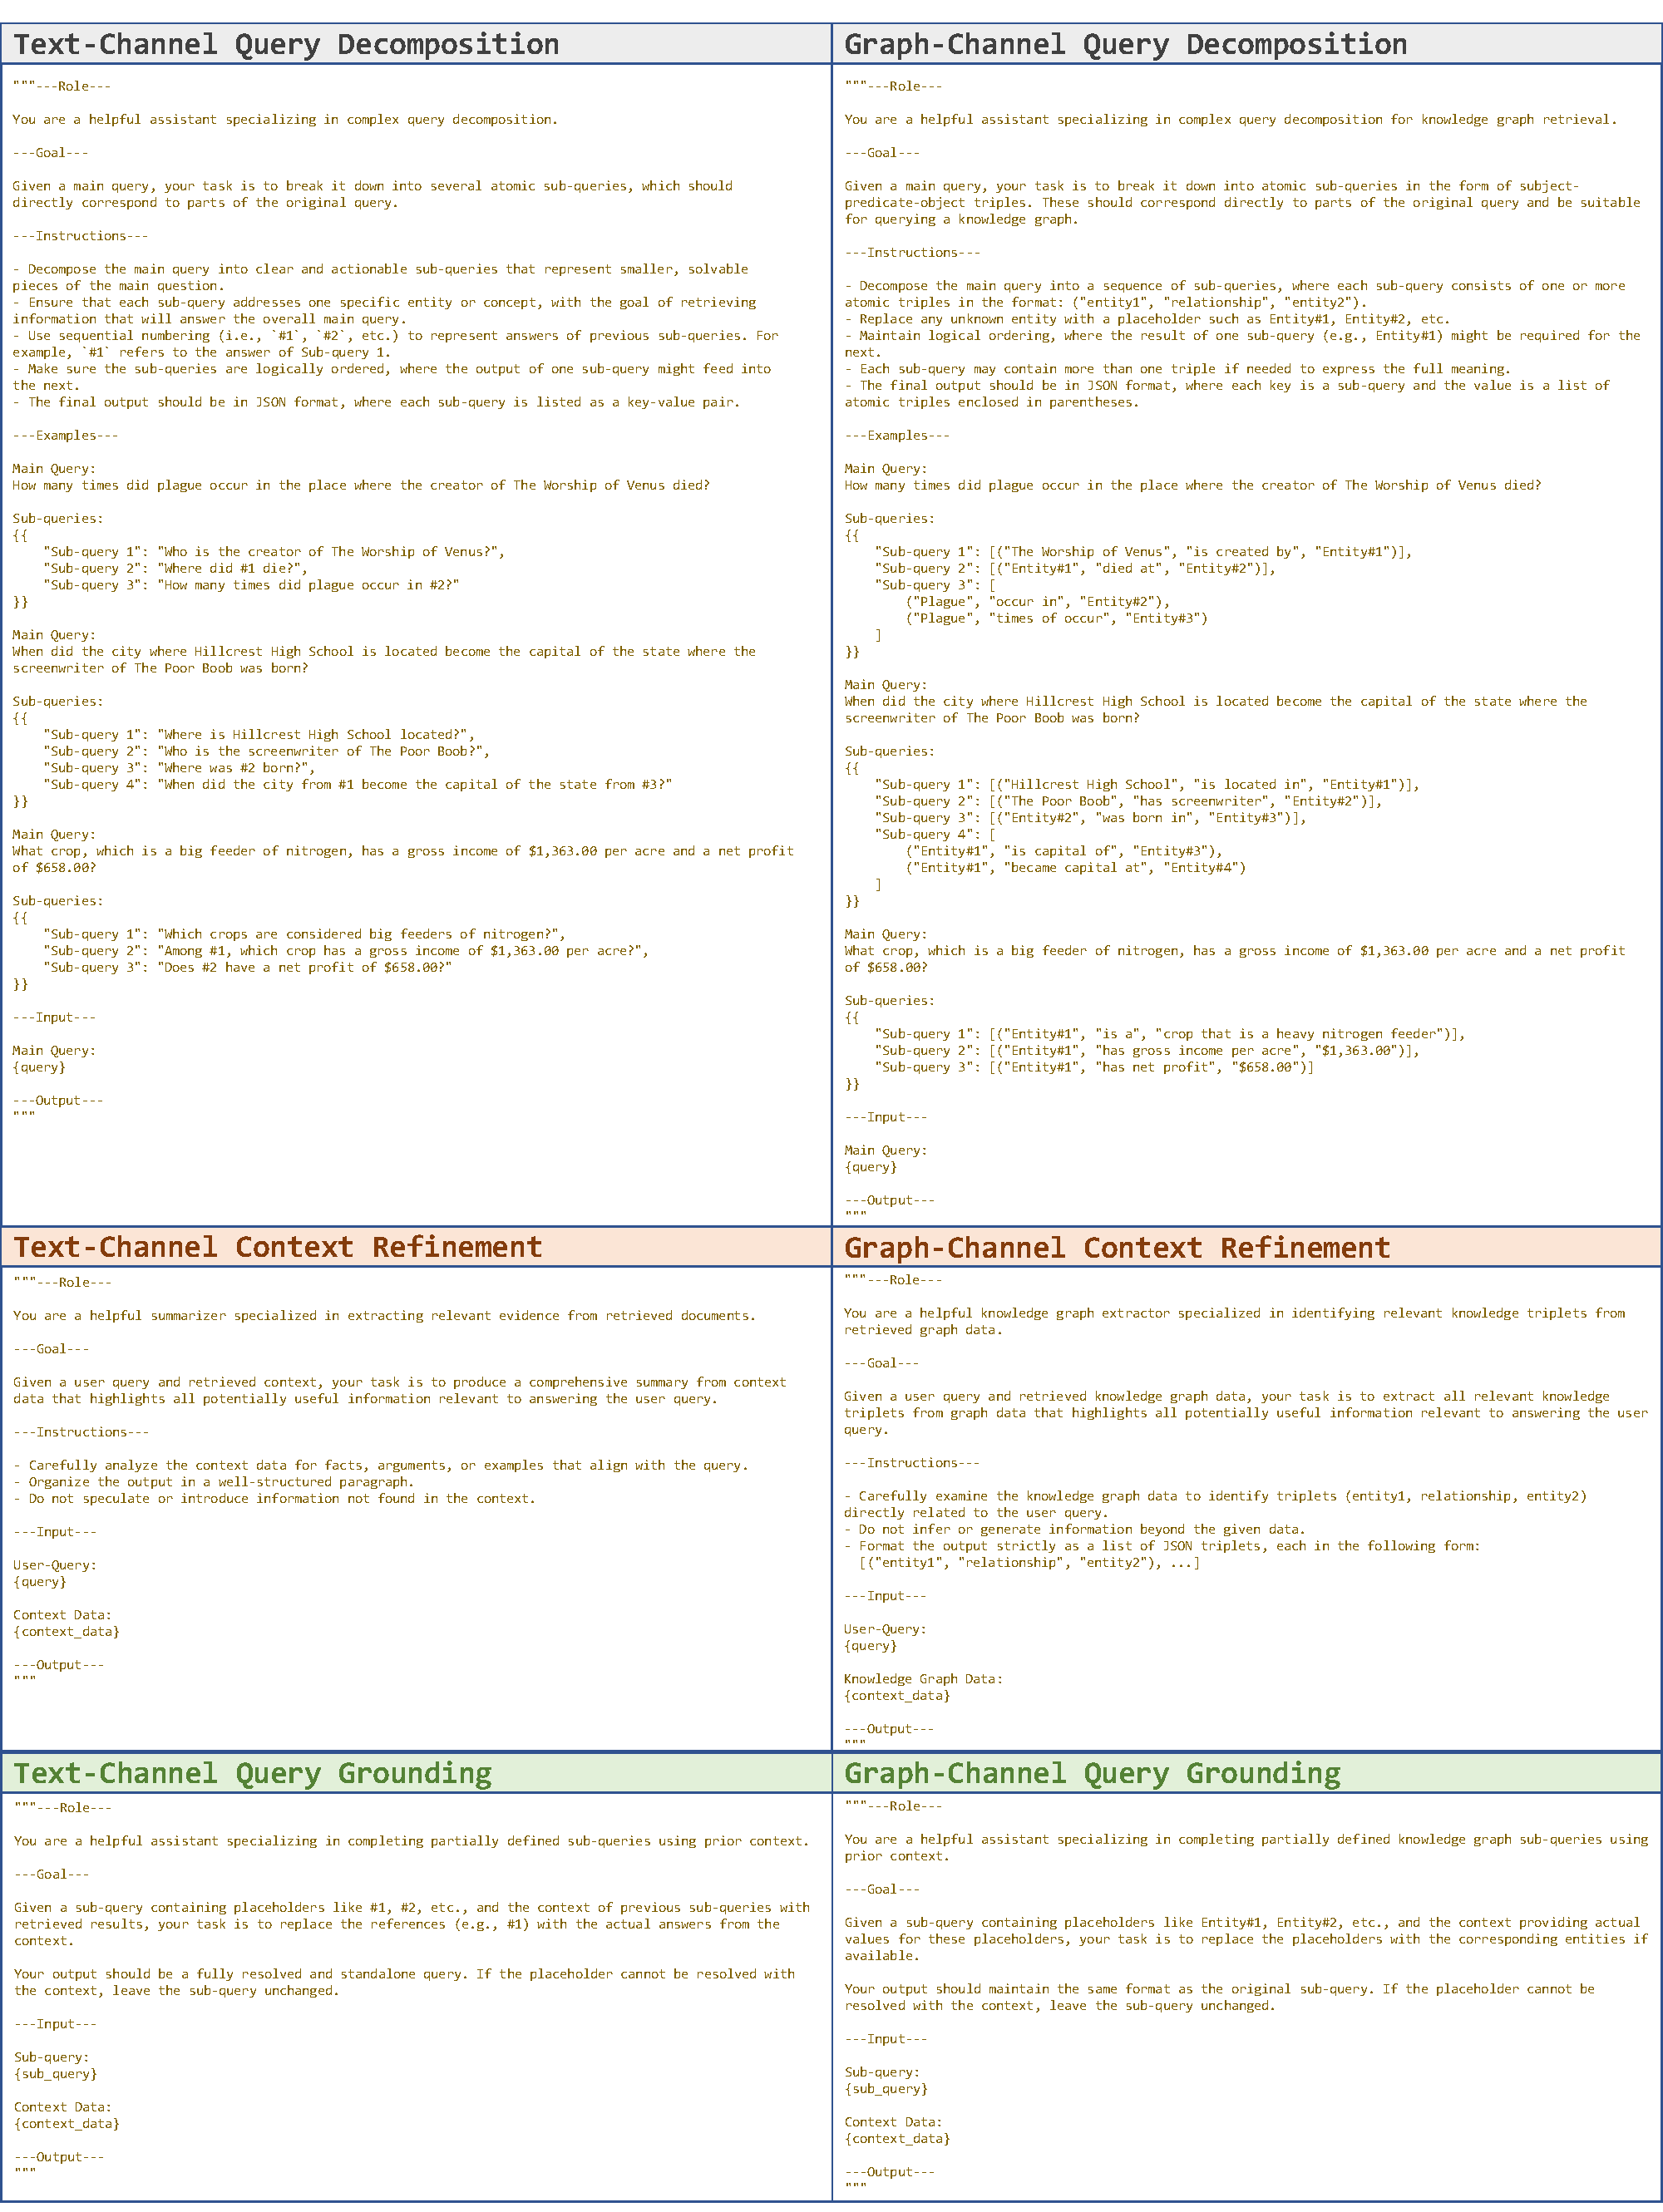
\includegraphics[width=\linewidth]{figs/prompt_1.pdf}
\caption{\label{fig:prompts_1}
Prompt templates of \textbf{Query Decomposition}, \textbf{Context Refinement} and \textbf{Query Rewriting} modules both in text-channel and graph-channel.}
\end{figure}

As shown in Figure~\ref{fig:prompts_2}, we introduce the prompt templates in \textbf{Logic Drafting}, \textbf{Evidence Verification} and \textbf{Query Expansion} modules for combining into a reflection router.

\begin{figure}[ht]
\centering
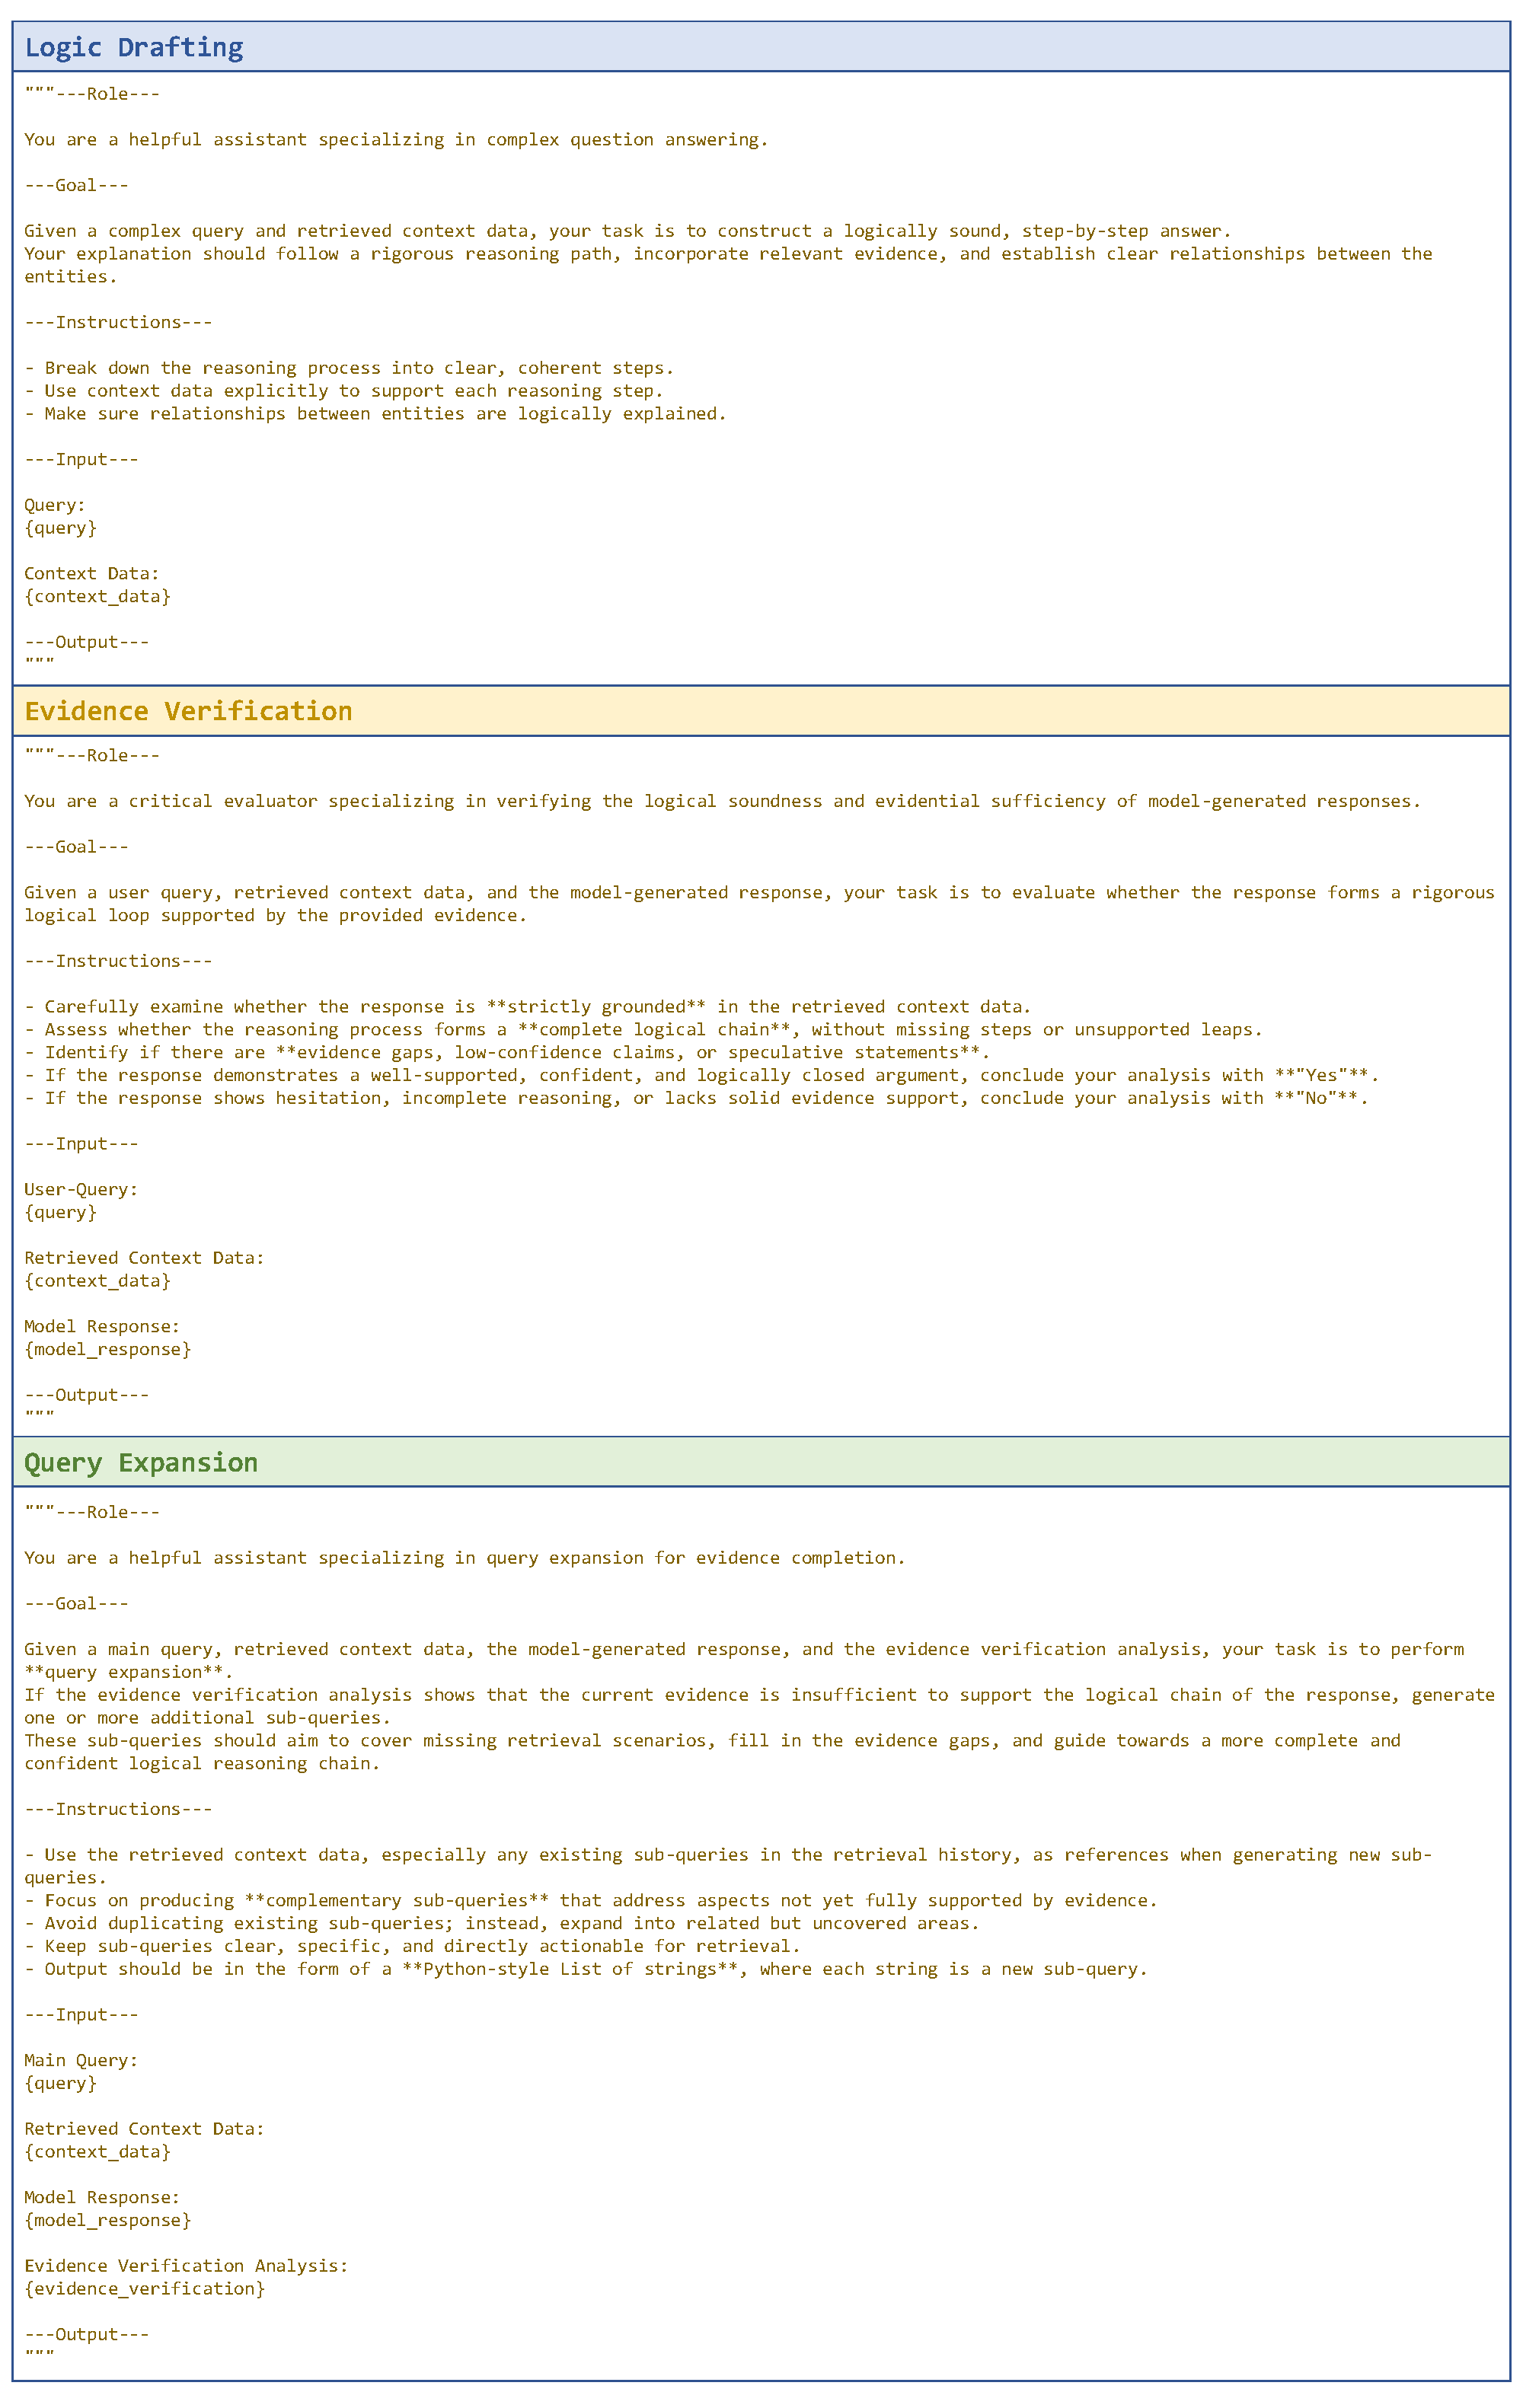
\includegraphics[width=0.90\linewidth]{figs/prompt_2.pdf}
\caption{\label{fig:prompts_2}
Prompt templates of \textbf{Logic Drafting}, \textbf{Evidence Verification} and \textbf{Query Expansion} modules for combining into a reflection router.}
\end{figure}

\section{Case Studies}
\label{app:case_study}
As shown in Figure~\ref{fig:case_baseline}, there are some cases of baseline methods, including vanilla LLM generation, Naive RAG and LightRAG. A case of our proposed \textsc{GraphSearch} is in Figure~\ref{fig:case_graphsearch}.

\begin{figure}[ht]
\centering
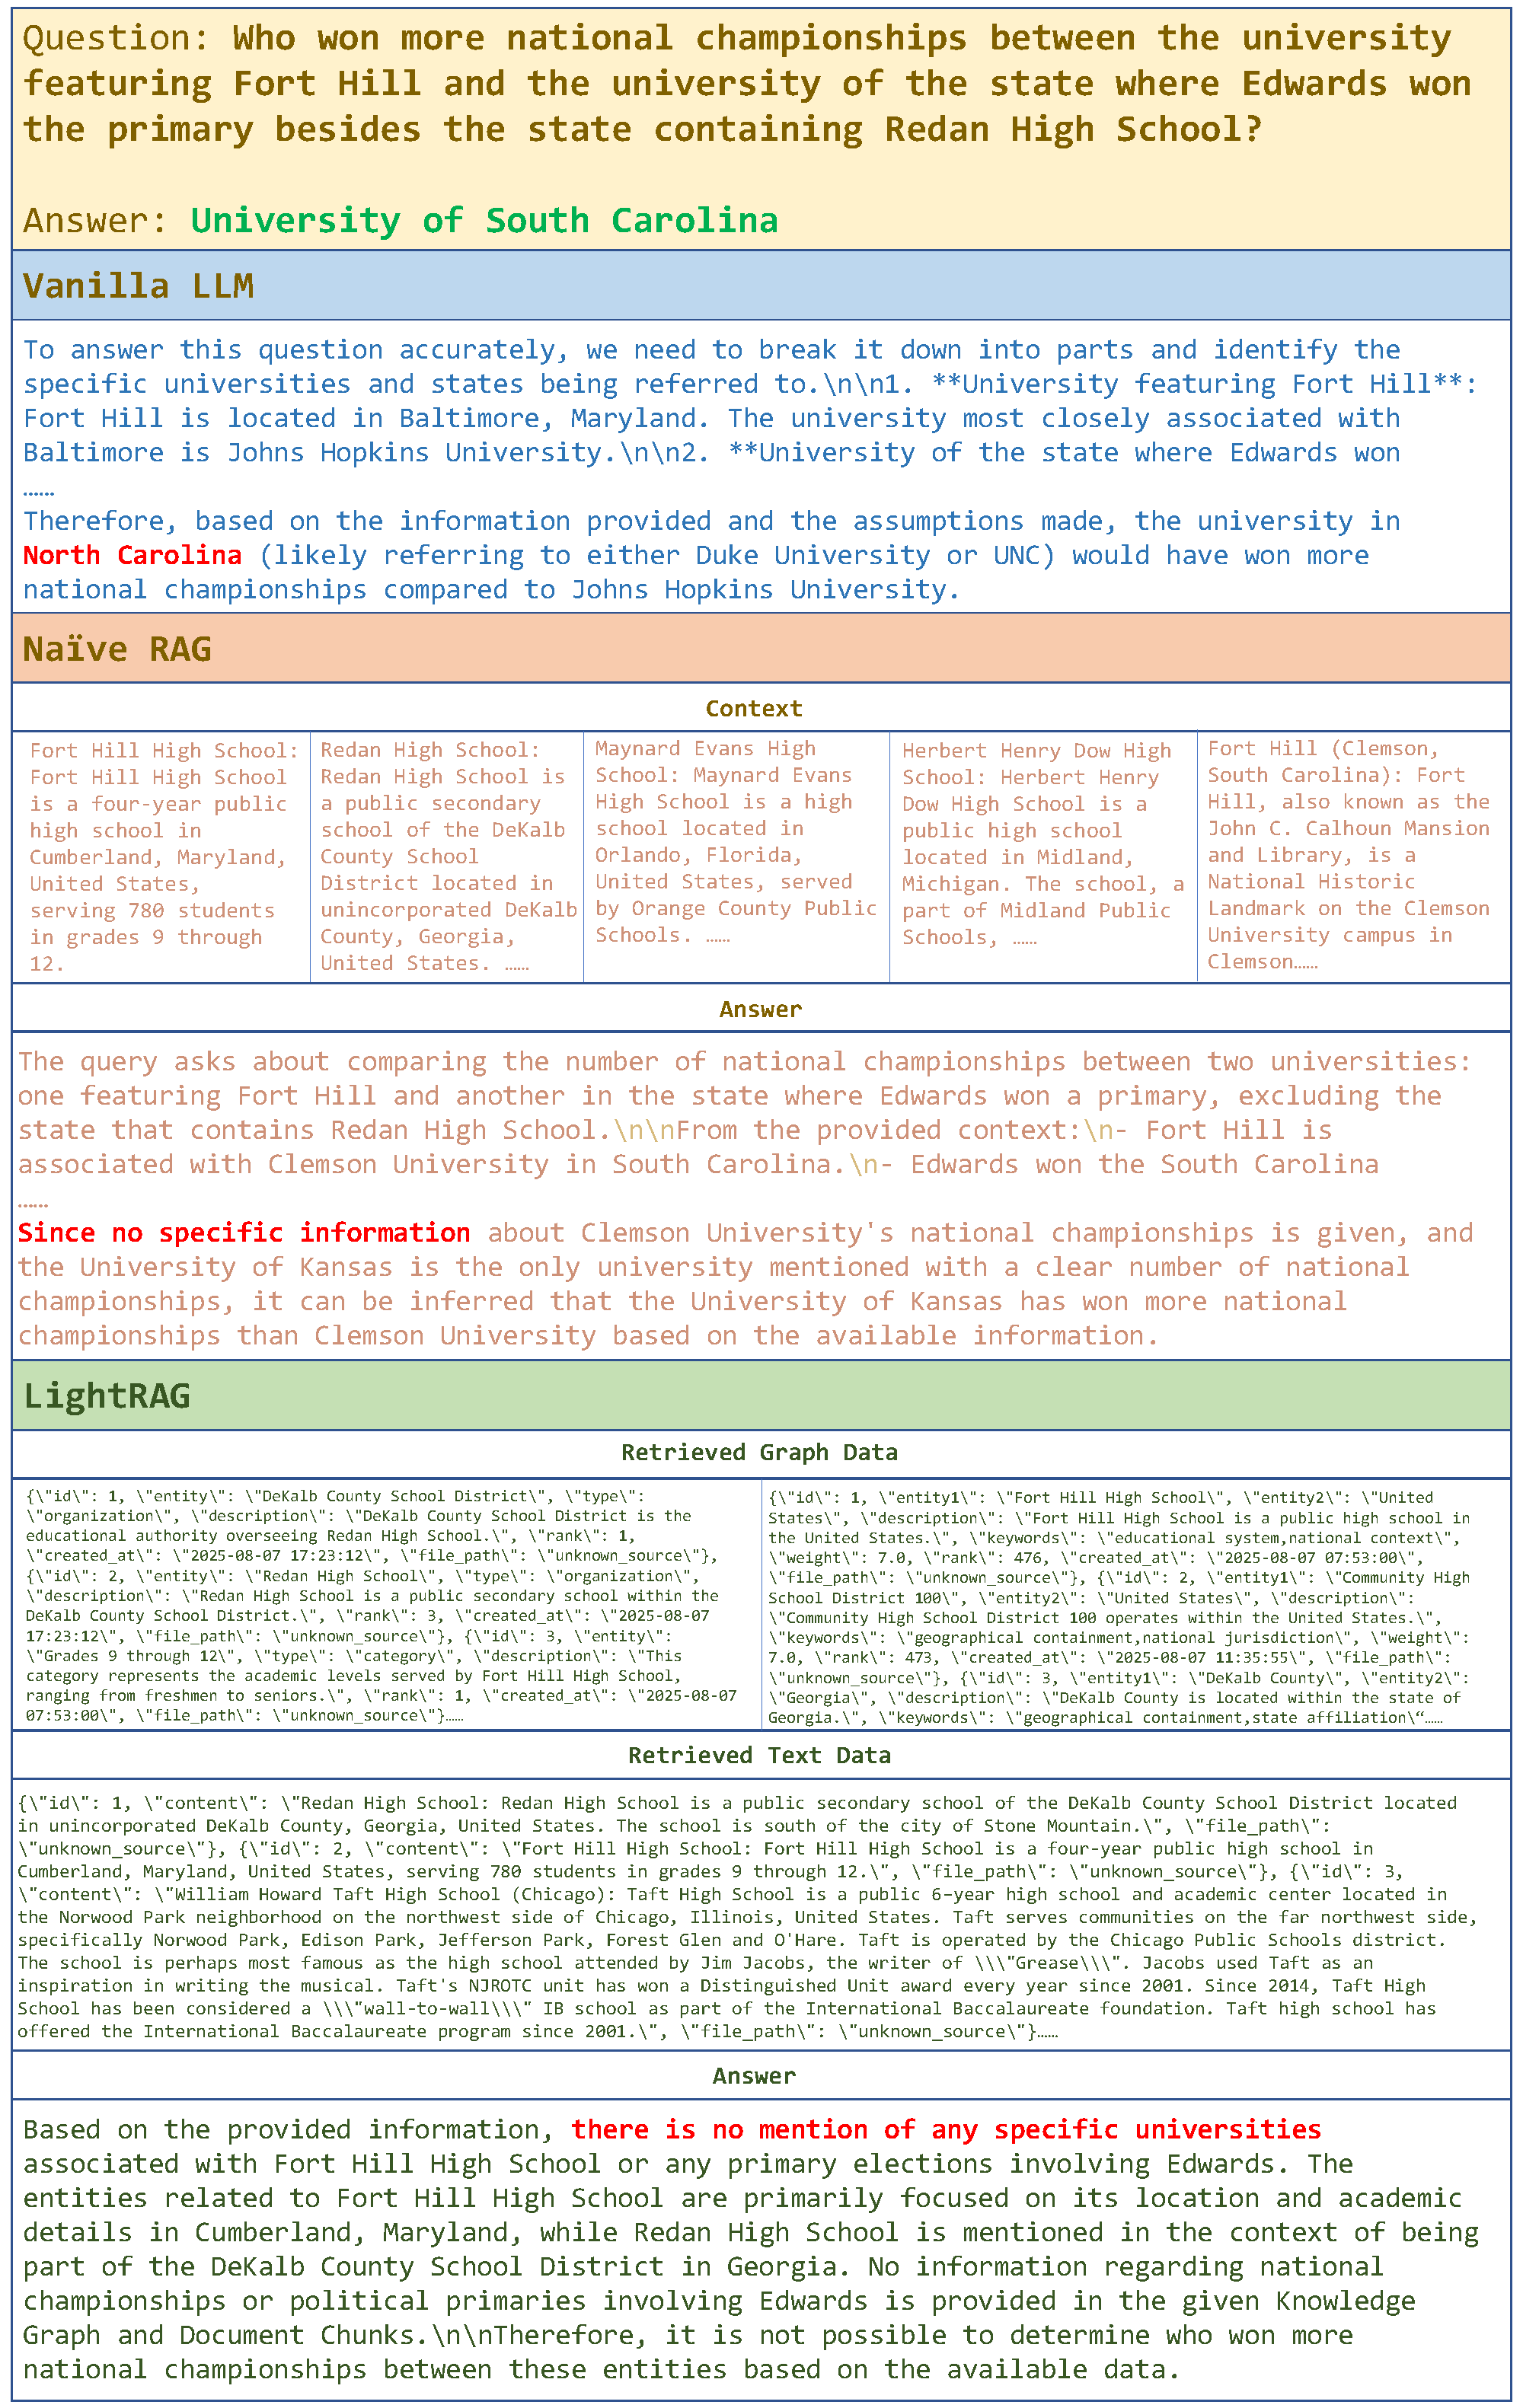
\includegraphics[width=0.9\linewidth]{figs/case_baseline.pdf}
\caption{\label{fig:case_baseline}Samples of Vanilla Generation, Naive RAG and LightRAG.}
\end{figure}

\begin{figure}[ht]
\centering
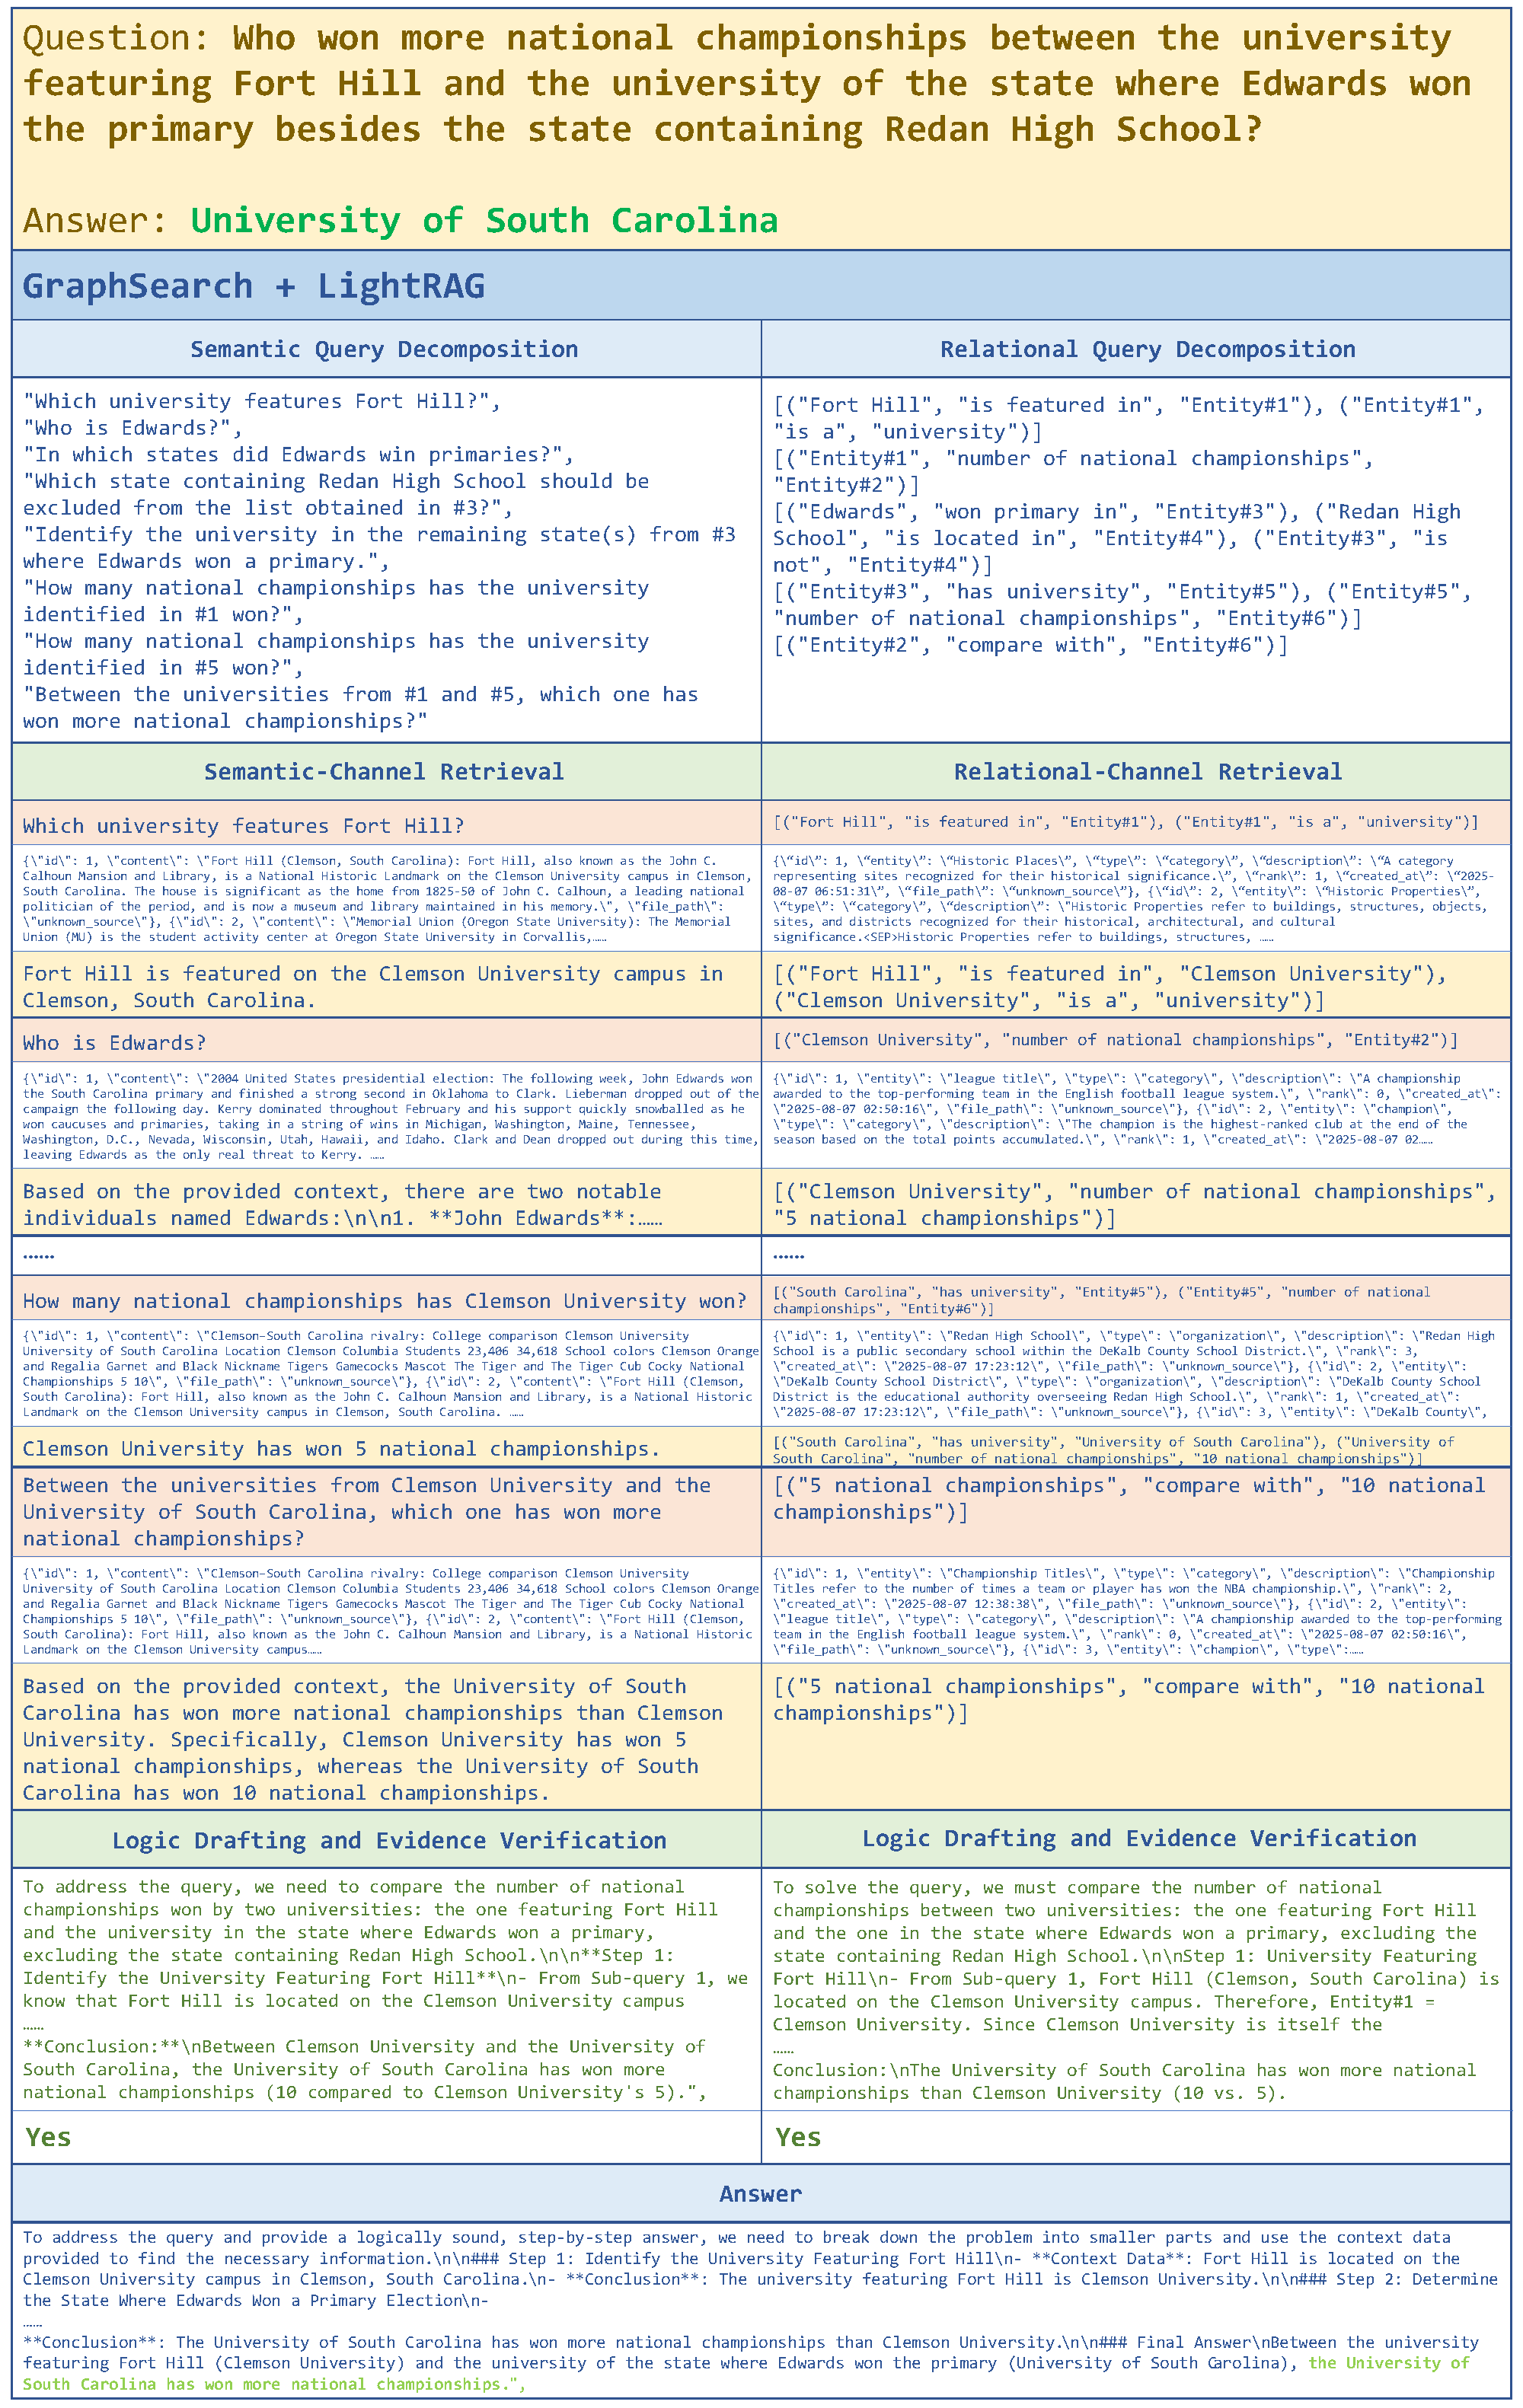
\includegraphics[width=0.9\linewidth]{figs/case_graphsearch.pdf}
\caption{\label{fig:case_graphsearch}A sample of \textsc{GraphSearch} with LightRAG as the graph retriever.}
\end{figure}

\section{Datasets}
\label{app:datasets}
As shown in Table~\ref{Tab:dataset}, we sample 300 questions for HotpotQA, MuSiQue and 2WikiMultiHopQA datasets, and directly adopt the Medicine, Agriculture and Legal datasets from~\citep{hypergraphrag}.

\begin{table}[ht]
\centering
\label{Tab:dataset}
\caption{Detail information of datasets used in \textsc{GraphSearch}. The tokenizer used to calculate the size of corpora is GPT-4o. \# means the number of counts.}
\scriptsize
\setlength{\tabcolsep}{4pt}
\begin{tabular}{lcccccc}
\toprule
\textbf{Name} & \textbf{Reference} & \textbf{Source} & \textbf{\#Corpus} & \textbf{\#Questions} & \textbf{Question Types} & \textbf{\#Evidence} \\
\midrule
HotpotQA          & ~\citep{hotpotqa} & Wikipedia & 397,274  & 300  & Comparison, Bridge  & 2,3,4     \\
MuSiQue           & ~\citep{musique} & Wikipedia & 533,145  & 300  & 2-Hop, 3-Hop, 4-Hop  & 2,4     \\
2WikiMultiHopQA   & ~\citep{2wiki}  & Wikipedia & 220,295  & 300  & Compositional, Comparison,   &  2,4    \\
 & & & & & Bridge Comparison, Inference & \\
Medicine          & ~\citep{medicine} & ESC Guidelines & 175,216  &  512 & 1-Hop, 2-Hop, 3-Hop  &   1,2,3   \\
Agriculture       & ~\citep{ultradomain} & UltraDomain & 378,592  &  512 & 1-Hop, 2-Hop, 3-Hop  &   1,2,3   \\
Legal             & ~\citep{ultradomain} & UltraDomain & 929,396  &  512 & 1-Hop, 2-Hop, 3-Hop  &   1,2,3   \\
\bottomrule
\end{tabular}
\end{table}

\section{Baselines}
\label{app:baselines}

\begin{itemize}[leftmargin=*]
\item \textbf{Vanilla LLM}: Zero-shot question and answering without any external retrieval source, depending on language model's parametric knowledge. 
\item \textbf{Naive RAG}~\citep{rag}: Generation with plain text chunk-based embedding database as external retrieval source, where top-k items are retrieved for a single round.
\item \textbf{GraphRAG}~\citep{graphrag}: A graph-based approach to question answering over hierarchical graph index where community summary is generated to represent the relationships.
\item \textbf{LightRAG}~\citep{lightrag}: A simple and fast GraphRAG framework by applying integration of graph structures with vector representations for a dual-level retrieval system.
\item \textbf{MiniRAG}~\citep{minirag}: A novel GraphRAG system designed for small LLM which adopts a lightweight topology-enhanced retrieval approach.
\item \textbf{PathRAG}~\citep{pathrag}: A GraphRAG system which retrieves key relational paths from the indexing graph through flow-based pruning.
\item \textbf{HippoRAG2}~\citep{hipporag2}: A RAG framework built upon the personalized PageRank with deeper passage integration.
\item \textbf{HyperGraphRAG}~\citep{hypergraphrag}: A novel hypergraph-based RAG method that represents n-ary relational facts via hyper-edges for retrieval and generation.
\end{itemize}

\section{Implementation Details.}
\label{app:implementation}
We conduct experiments on a Linux server equipped with 8 A100-SXM4-40GB GPUs. The model for graph construction is \textit{Qwen2.5-32B-Instruct}, and the chunk size is $400$ tokens. The embedding model for Naive-RAG and GraphRAG is \textit{jinaai/jina-embeddings-v3}~\citep{jina}. For \textsc{GraphSearch} and baselines, we set the \textbf{Hybrid} retrieval mode and set the \textbf{Top-K} for retrieval to $30$, or use the default configuration if unavailable. The backbone model for generation is \textit{Qwen2.5-7B/32B-Instruct}~\citep{qwen}. The LLM-as-a-Judge for evaluation is \textit{Qwen-Plus}~\citep{qwen}, a strong closed-source model with API available.

\section{Evaluation Details}
\label{app:evaluation}
Inspired by~\citep{longfaith, hypergraphrag}, we leverage the Substring Extract-Match(\textbf{SubEM}) metric to check whether the golden answer is explicitly contained in the response, the Answer-Score(\textbf{A-Score}) to judge the quality of model generation across 3 criteria covering \textbf{correctness}, \textbf{logical coherence} and \textbf{comprehensiveness} with the \textbf{golden answer} as reference, and the Evidence-Score(\textbf{E-Score}) to measure how well the model’s generation is grounded in the golden evidence, evaluated along 3 criteria including \textbf{relevance}, \textbf{knowledgeability} and \textbf{factuality} with the \textbf{golden evidence} as reference as follows:

\begin{equation}
\text{SubEM} = \frac{1}{N} \sum_{i=1}^{N} 
\mathbf{1}\!\left[ \text{contains}\!\left(O^{\text{pred}}_{i}, A^{\text{gold}}_{i}\right) \right],
\end{equation}

\begin{figure}[ht]
\centering

\includegraphics[width=\linewidth]{figs/evaluation.pdf}
\caption{\label{app:eval_prompt}
Evaluation prompts of \textbf{A-Score} across 3 criteria and \textbf{E-Score} across 3 criteria.}
\end{figure}

\section{Limitations and Future Direction}
Although \textsc{GraphSearch} has made progress in advancing \textsc{GraphRAG}, there are still some limitations. First, it remains uncertain whether \textsc{GraphSearch} can unlock greater potential under different training strategies, such as fine-tuning or reinforcement learning. Second, how to integrate it with cutting-edge reasoning models is still an open question. Finally, applying \textsc{GraphSearch} to scenarios involving multimodal corpora is a direction worthy of further investigation.

% \section{The Use of Large Language Models (LLMs)}
% During the completion of this thesis, the scenarios involving the use of LLMs included: using code-completion tools to assist with experiments, and using ChatGPT to polish the draft after the initial writing was completed. LLMs were not involved in any aspects such as the development of research ideas, literature review, and so on.